\documentclass{report}

\usepackage[utf8]{inputenc}
\usepackage[T1]{fontenc}
\usepackage[francais]{babel}
\usepackage{setspace}
\usepackage{listings} 
\usepackage{hyperref}
\usepackage{amssymb}
\usepackage{graphicx}

\begin{document}
\lstset{language=C}

\title{Synthèse finale du projet de jeu 2048}
\author{Guillaume ALMYRE 
\and
Ga\"{e}tan CHAMBRES
\and
Allan MAHAZOASY
\and 
Chrystelle PETUREAU}
\date{21/04/2015}

\maketitle

\tableofcontents

\chapter{Notre projet:Le 2048 jouable en 3 mode!}
Nous avons créé un programme en langage C qui permet de jouer au jeu "2048" soit en mode terminal, soit avec une interface graphique. Il y a aussi 2 stratégies, une rapide et une efficace, pour qu'une intelligence artificielle joue à la place de l'utilisateur.

\section{Le contenu du dossier}
Cette première section présente les différents fichiers présents dans le dossier. Le temps approximatif que nous avons passé à créer chaque fichier est noté entre parenthèses. Notre travail est décrit plus précisément dans les sections suivantes.\\
\begin{description}
\item [README (1 heure):] ce ficher est le résumé de ce rapport. Il permet d'expliquer à l'utilisateur comment utiliser notre dossier. Un ton un peu humoristique a été utilisé pour rappeler l'ambiance "bon enfant" de certains jeux vidéo.
\item[Makefile (3 heures):] Il permet de compiler le jeu en utilisant la commande "make". dans le terminal. Le plus long dans ce fichier a été d'arriver à trouver la ligne pour créer la bibliothèque libgrid et de compiler avec. Ce fichier n'est utile que pour le mode "terminal". Les ligne de commande pour les autres modes sont données dans le fichier README.
\item[gric.h:] Il s'agit de l'interface du jeu, à laquelle nous n'avons absolument pas touché.
\item[grid.c (45 heures):] Il constitue le code principal du programme. 
\item[test-grid.c (8 heures):] C'est le fichier où tous les tests ont été effectués.
\item[jeu.c (6 heures):] C'est le fichier pour créer l'exécutable pour jouer en mode "terminal".
\item[dossier stratégie (23 heures):] Ce dossier regroupe tous les codes pour les intelligences artificielles. Les 2 bibliothèques dynamiques ainsi que le fichier tournament sont mis dans le dossier principal pour permettre à l'utilisateur d'organiser de suite un tournois comme expliqué dans le README.
\item[graph.c (8 heures):] Il constitue le code pour le mode graphique. Il est étroitement lié aux dossiers fonts qui gère les polices de ce mode et sprites qui gère les images de fond.
\item[dossier fichier lateX (9 heures):] qui contient toutes les synthèses de notre projet.
\end{description}

\section{La répartition du travail}

Notre groupe, au départ,le 27 janvier, était constitué de 3 personnes. Il a finalement été agrandi à 4 personnes, le 10 mars, avec l'arrivée d'Allan.\\ Nous nous sommes répartis le travail en fonction de notre savoir-faire ainsi que de nos avis. Gaëtan et Guillaume ont beaucoup travaillé sur l'implémentation de grid.c et strategie.c. Chrystelle sur test-grid.c ainsi que tous les comptes rendus. Grâce à ce découpage, il y a eu presque deux équipes au sein du projet. Cela nous a permis de travailler sur la lisibilité du code: si une équipe arrive à comprendre et utiliser le code sans y avoir participé, cela veut dire que le code est lisible et bien commenté.\\ Allan a essayé de "prendre le train en marche" avec beaucoup de bonnes volontés. Nous l'avons aidé du mieux qu'on a pu mais il n'avait jamais codé en C, ne connaissait pas le jeu 2048 et était très peu présent en cours donc son travail n'a pas été significatif. On ne peut donc pas réellement montrer son travail dans ce rapport.
\section{Les outils utilisés}
Dès le début du projet,nous avons créé un framapad. Nous l'avons initialisé avec le contenu du PDF "sujet" puis mis à jour à chaque modification. Cet outil a été d'une grande aide. Il nous a permis au fur et à mesure de savoir sur quelle partie du code travailler, les modifications faites par chacun et les pistes à travailler. \\
Nous avons également utilisé un serveur github. L'adresse du dépôt utilisé est: \url{https://github.com/projetL2/2048.git} \\Les identifiant sont :
\begin{description}
\item [username : ] projetL2
\item [password : ] IN400A1ggc  (pour Guillaume, Gaëtan, Chrystelle)
\end{description}
La fonction "historique" du framapad ainsi que celle du serveur github ont été d'une grande aide pour retrouver les étapes de notre travail et surtout le temps passé dessus, afin de faire un rapport objectif et détaillé.

\chapter{Le mode terminal}
Ce mode de jeu permet de jouer dans le terminal avec les touche haut, bas, droite et gauche du clavier de façon simple mais efficace.
\section{Le coeur du programme: grid.c}
Ce fichier contient la structure de base de notre programme. Un pointeur de pointeur qui donne la matrice pour la grille et un unsigned long int pour le score.
\begin{lstlisting}[frame=single]
struct grid_s {
unsigned long int score;
tile** grid;
};
\end{lstlisting}

Il contient aussi toutes les fonctions obligatoire pour ce type de jeu:\\

\begin{description}
\item [new-grid :] Le constructeur de la grille. Il initialise le score à 0 et fait les allocations mémoire nécessaires pour la structure de la grille.
\item [delete-grid :] Le destructeur de la grille. Il libère d'abord les zones de la mémoire pointées par la variable grid puis la grille elle-même.
\item [copy-grid :] C'est un constructeur par copie de grid.
\item [grid-score :] L'accesseur qui retourne le score de la grille.
\item [get-tile :]  L'accesseur qui retourne une tuile en fonction des coordonnées passées en paramètre.
\item [set-tile :] L'accesseur qui modifie la valeur d'une tuile en fonction des coordonnées et de la valeur passées en paramètre.
\item [can-move :] C'est une fonction de type booléenne. Elle renvoie true si le joueur peut effectuer le mouvement dans la direction passée en paramètre et false dans le cas inverse.
\item [game-over :] Cette fonction booléenne renvoie true si aucun mouvement n'est plus possible.
\item [do-move :]Cette fonction permet de déplacer toutes les tuiles suivant la direction passée en paramètre.
\item [add-tile :] Cette fonction ajoute une tuile de façon aléatoire dans une case vide de la grille. On se sert de la fonction random pour cela.
\item [play :]Contrairement à son nom, cette fonction permet juste de vérifier que la direction donnée par le joueur est valide, de l'effectuer et d'ajouter une nouvelle tuile. La boucle de jeu est en réalité dans les fichier test-grid.c , jeu.c, graph.c et dans les bibliothèques dynamiques. Cette apparente duplication a en réalité permit d'adapter la boucle au mode de jeu demandé.\\ De même, la fonction afficher est présente dans jeu.c et test-grid.c car nous ne voulions pas ajouter de fonctions au fichier grid.h donné.
\end{description}
\begin{figure}[hbtp]
\caption{affichage d'une grille vide}
\centering
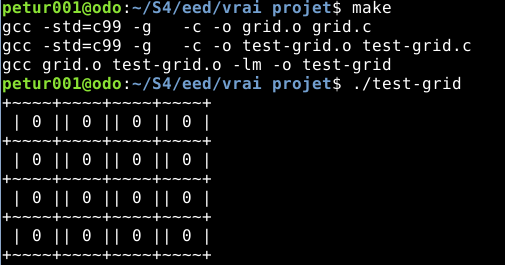
\includegraphics[scale=0.6]{1ergrille.png}
\end{figure}
\section{La partie jouable: jeu.c}
Grâce à l'utilisation de la bibliothèque "ncurses", nous avons pu crée une boucle de jeu qui transforme une grille en chaîne de caractères. La bibliothèque ncurses permet de les afficher. Les lignes de commande:
\begin{lstlisting}[frame=single]
initscr(); 
keypad(stdscr, TRUE);
\end{lstlisting}
permettent d'initialiser la bibliothèque et d'activer les événements clavier.\\
Nous avons choisi l'utilisation des touches haut,bas,droite et gauche du clavier pour le déplacement. Cela nous semblait être le choix le plus intuitif. Les touches Z,Q,S,D sont très utilisé par les gamers. Cependant, cette communauté ne représente pas la totalité des joueurs du 2048.

\chapter{Le mode graphique}
Nous avons créé un mode graphique pour jouer de façon plus plaisante.Pour cela nous avons utilisé la bibliothèque SDL2.
\begin{figure}[hbtp]
\caption{affichage d'une grille en mode graphique}
\centering
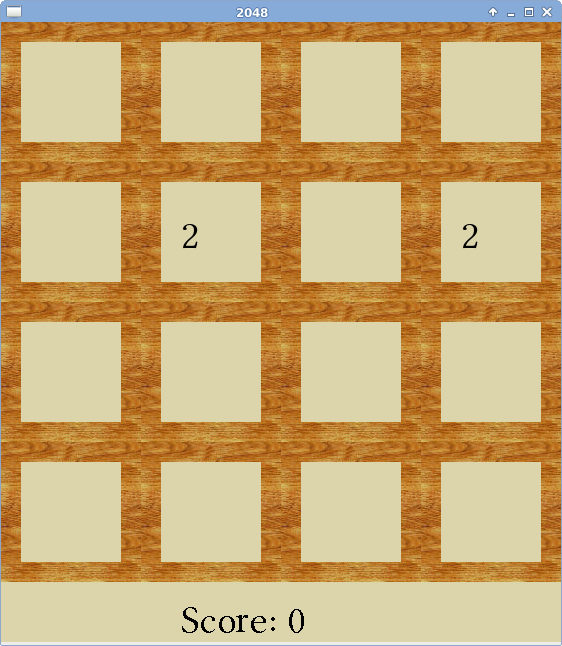
\includegraphics[scale=0.3]{modegraphique.png}
\end{figure}
\section{Notre idée de base}
Pour commencer notre interface graphique, nous nous sommes fixé comme objectif principal de pouvoir adapter notre fenêtre à la taille de la grille donnée par la variable GRID-SIDE dans le fichier grid.h. Pour cela, nous avons abandonné la solution de facilité qui consiste à afficher une grille vide trouvée sur le net en fond de fenêtre.\\
Nous avons créé nous même un carré de tuile et nous l'avons dupliqué GRID-SIDE fois en longueur et en largeur.\\
Nous avons choisi de créer une tuile de 140 * 140 pixels. Une bordure de 20 pixels est ajouté de chaque cotés.\\
Pour créer notre fenêtre de jeu, nous avons initialisé 2 variables représentant la longueur et la largeur de la fenêtre :
\begin{lstlisting}[frame=single]
#define SCREEN_WIDTH (GRID_SIDE*140)
#define SCREEN_HEIGHT (GRID_SIDE*140)+60
\end{lstlisting}
Les 60 pixels ajoutés en bas de l'image permettent de garder la place d'afficher le score.\\
\section{Les fonctions créées}
Nous avons partagé le code en plusieurs fonctions:
\begin{description}
\item[bool init() :] cette fonction permet l'initialisation de SDL2, et elle nous renvoie un booléen, false s'il y a eu un problème à l'initialisation, true dans le cas inverse.
\item[nouveauJeu(SDL-Surface* surface) :] Cette fonction permet de couvrir la surface passée en paramètre avec la couleur RGB = (220, 212, 171). Cette dernière est la couleur pour le fond des tuiles. Le fait de recouvrir la surface de fond par la couleur (220,212,171) permet que l'affichage du score se fasse sur le même fond que celui des tuiles.\\
Cette fonction remplie enfin cette surface du nombre de tuiles nécessaire grâce à la boucle suivante:
\end{description}
\begin{lstlisting}[frame=single]
for(int i = 0; i<GRID_SIDE; i++)
        for (int j=0; j<GRID_SIDE; j++) {
            tmp.x=i*140;
            tmp.y=j*140;
            SDL_BlitSurface(tile,NULL,surface,&tmp);
        }
\end{lstlisting}
\begin{description}
\item[void dessinerGrille(SDL-Surface* surface, grid g) :] Cette fonction crée une surface supplémentaire qui contient les valeurs de la grille et l'affichage du score. Cette fonction  parcours la grille et inscrit sur la surface les valeurs des tuiles. Pour trouver les coordonnées x et y de la tuile on utilise le code suivant:
\end{description}
\begin{lstlisting}[frame=single]
pos.x = 40 + (140*colonne);
pos.y = 50 + (140*ligne);
\end{lstlisting}
Les variables x = 40 et y = 50 donnent la position dans la tuile. Les variables x = 140 * colonne et y = 140 * ligne donnent, quant à elles, le placement de la tuile concernée.\\
Cette fonction gère aussi le game-over et affiche, par dessus la surface, une nouvelle surface qui contient le mot "Game-Over" écrit en plein milieu.
\begin{description}
\item[int main() :] Cette fonction est la fonction principale. Elle gère l'ensemble de l'affichage de la fenêtre.\\
Elle commence par appeler init. Cette fonction vérifie que l'initialisation a été faite correctement. Elle initialise ensuite la fonction rand et crée une nouvelle grille en lui ajoutant 2 tuiles.\\
Elle crée une fenêtre de la taille SCREEN-WIDTH * SCREEN-HEIGHT et donne à la surface le contenu de cette fenêtre. La fonction main appelle ensuite la fonction nouveauJeu qui rempli le fond de la fenêtre.\\
La gestion des évènements claviers et de la touche "quit"  se font à l'aide du switch suivant:
\end{description}
\begin{lstlisting}[frame=single]
while(!quit) {
	SDL_Event e;
	while(SDL_PollEvent(&e)) {
    	switch(e.type) {
        	case SDL_QUIT :
                quit = 1;
                break;
                case SDL_KEYDOWN :
                    switch( e.key.keysym.sym ){
                    case SDLK_LEFT:
                        play(g,LEFT);
                        break;
                    case SDLK_RIGHT:
                        play(g,RIGHT);
                        break;
                    case SDLK_UP:
                        play(g,UP);
                        break;
                    case SDLK_DOWN:
                        play(g,DOWN);
                        break;
                    default:
                        break;
                    }
        break;
        }
\end{lstlisting}
Tant que l'on n'a pas cliqué sur l'icône "quit",Le jeu attend un évènement clavier. Si c'est une touche directionnelle, on joue la direction demandée.\\
On libère la surface, on dessine la nouvelle grille sur la surface, et on met à jour l'affichage grâce aux appels respectifs des fonctions suivantes:\\
\begin{lstlisting}[frame=single]
SDL_FreeSurface(surface);   
dessinerGrille(surface, g);
SDL_UpdateWindowSurface( fenetre );
\end{lstlisting}
Pour finir, lorsque l'on quitte la fenêtre, la fonction main s'occupe de libérer la mémoire en libérant la font, puis la surface, en détruisant la fenêtre et enfin en quittant SDL2:
\begin{lstlisting}[frame=single]
TTF_CloseFont(font);
SDL_FreeSurface(surface); 
SDL_DestroyWindow(fenetre); 
SDL_Quit();
\end{lstlisting}

\chapter{Les Intelligences Artificielles}
Ce mode de jeu ne permet pas de jouer. C'est une intelligence artificielle qui joue à la place de l'utilisateur.
\section{Les deux stratégies}
Le fichier strategy.h est la base de tout notre travail sur ce mode de jeu. Nous ne l'avons absolument pas modifié. On a défini une structure pour chaque stratégie. Cette structure contient: un nom sous forme de char*, une variable qui mémorise les moments, un pointeur de fonction qui applique la stratégie et trouve la direction à effectuer et enfin un pointeur de fonction qui libère la mémoire (pour ne pas avoir de problème de mémoire pleine).\\
L'utilisation de pointeurs de fonctions permet de garder le code identique, sans changement de grid.c. Cela évite la création involontaire de bogues.\\
Donc, en résumer, pour chaque stratégie il y a en commun:
\begin{itemize}
\item Makefile
\item grid.h
\item grid.c
\item strategy.h
\item strategy.c\\
Pour simplifier le travail de compilation, il y a aussi:
\item grid.o
\item strategy.o\\
\end{itemize}
Seulement 3 fichiers sont différents suivant les stratégies: fast.h, fast.c ou efficient.h, efficient.c et leurs bibliothèques respectives.\\
Les fichiers fast.h et efficient.h sont obligatoires car nous avons créé un fichier test-strat pour tester ces stratégies. Les appels de test-strat à fast.c ou effecient.c doivent ce faire par le biais d'un .h. On trouve dans ce .h la signature d'un constructeur qui initialise la structure de la stratégie concernée. Il y a aussi la signature de la fonction qui applique la stratégie et retourne une direction.\\
Les tests sont faits à partir d'un simple copier-coller de "jeu.c" avec l'ajout de la ligne:
\begin{lstlisting}[frame=single]
strategy s=fastInit();
\end{lstlisting}
ou
\begin{lstlisting}[frame=single]
strategy s=efficientInit();
\end{lstlisting}

\subsection{La stratégie rapide}
Dans le fast.c, on trouve, comme prévu, un constructeur fastInit qui initialise la structure 's' ainsi qu'une fonction stratFast qui test les mouvements dans un ordre bien défini : droite, bas, gauche, haut. Le but étant d'avoir la plus grande valeur toujours en bas à droite mais surtout de jouer très vite les mouvements.\\
La création de cette fonction a été relativement facile (environ 3 heures), la compréhension du travail demandé et l'utilisation des pointeurs de fonctions étant beaucoup plus chrono-phage (environ 5 heures).
\subsection{La stratégie efficace}
Le principe de base est de chercher la direction qui minimise l'évaluation 'e' de la grille 'g'. La formule utilisée est:
$$e=2*L+2*US+6*M$$ avec:
$$L=\sum_{i=0}^{GRIDESIDE} .^{ } \sum_{f=0}^{GRIDESIDE}[|(t(i,j)-t(i-1,j))|+[t(i,j)-t(i,j-1)|]$$
$$US=card(t \in g / (t(i,j)>0 et i,j \in [0,grideside]) $$
$$M=min(sup(i),inf(i)) + min(sup(j),inf(j))$$
Dans cette stratégie, le plus compliqué a été de coder un tri de tableau efficace. L'application des cours d'algorithme du semestre 3 n'a pas été des plus facile!

\chapter{Les difficultés rencontrés}
Dans ce genre de programme, il y a toujours beaucoup de bogues. Nous allons, dans cette partie, essayer d'expliquer notre démarche pour les limiter aux maximum.
\section{Les tests effectués}
Nous avons choisi de créer des tests spécifiques pour chaque fonctions. Cela nous permettait d'être sûr de ne pas avoir de problèmes de dysfonctionnement dans nos fonctions.
\begin{description}
\item [afficher, set-tile et get-tile:] Ce sont les premières vraies fonctions qui ont été créées, elles sont vitales pour tester les autres. Depuis le début du projet, elles ont servit un nombre incalculable de fois sans jamais révéler aucun problème.
\item [new-grid :] nous l'avons testé dans le ficher test-grid.c. Ce test fait parti de la base des tests des autres fonctions. Aucun problème n'a été révélé sur cette fonction mais avec les tests d'autres fonctions par son bais.
\item [add-tile :] Son principal test est une boucle for avec new-grid, afficher et add-tile pour vérifier son aspect aléatoire.
\item [copy-grid :]Associée à la fonction afficher, les 2 grilles semblent tout à fait identique.
\item [delete-grid :] Nous avons crée un test avec new-grid, add-tile, copy-grid puis delete-grid. Ce fichier à été lancer avec valgrind pour vérifier les éventuelles fuites de mémoire. Les allocations sans libérations visibles sont du à l'utilisation de la bibliothèque ncurses.
\item [do-move :] Cette fonction est surtout testée dans une boucle for avec l'utilisation de la fonction random.
\item [grid-score et can-move :] Ces deux fonctions sont testées à chaque boucle.
\item [play et game-over:]Ces deux fonctions sont utilisées dans la boucle de jeu. 
\end{description}

\section{Les optimisations possibles}
Un vrai travail sur la suppression de duplication de code pourrait être fait dans notre projet. En effet, beaucoup de fichiers sont des copier-coller d'autres fichiers avec seulement quelques lignes de code qui changent.\\ Nous avons préféré nous concentrer sur un code lisible, commenté et efficace plutôt que sur des optimisations qui souvent créent des bogues. De plus, le jeu à été créé par étapes et, donc ,sans réel réflexion sur l'ensemble et le résultat final. Nous avons donc un code moins optimisé que d'autres groupes mais il est sans dysfonctionnement.\\
Une autre piste d'évolution serait de créer des tests automatiques. Ces derniers pourraient permettre d'être sûr que le jeu est fiable sur d'autres configurations que celles du Cremi.\\
L'initialisation avec 2 tuiles dans le mode terminal devra être rajouter aussi. Nous ne connaissions pas cette règles du 2048 lors de la fin de la première partie.

\chapter{Notre avis sur les outils proposés}

\section{Makefile ou Cmake?}
Toute l'année de L1 ainsi que le semestre dernier nous avons rêvé d'un logiciel qui crée les Makefile automatiquement, ces derniers étant vraiment compliqués à créer surtout dans la bonne utilisation des variables. Cependant, à force de persévérance, nous avons réussi à créé un Makefile "type" que nous utilisons dans tous les projets. Après le test de Cmake effectué par la feuille de TP 2, nous avons décidé de garder notre Makefile car il semble finalement plus simple à utiliser et ne demande pas d'avoir Cmake d'installer sur l'ordinateur. Enfin, il crée une archive beaucoup plus propre.

\section{L'utilisation d'un serveur? SVN ou git?}
Après avoir fait les tests de SVN et GIT de la feuille de TP3, nous avons choisi de privilégier Git par rapport à Subversion car cet outil nous  semblait plus intuitif. Après quelques mois d'utilisation, on ne voit plus comment se passer de ce genre de serveur pour n'importe quel type de projet à plus de 1 personne. Nous avons pris l'habitude d'en créer un pour tout projet à plusieurs.\\
Nous tenons à souligner que l'utilisation de ce type de serveur en ligne est tout à fait complémentaire de l'utilisation d'un framapad par exemple. Ces genres d'éditeurs de texte en ligne permettent de commenter le travail qu'on a faire, le but, les pistes à suivre, ce qu'il reste à faire. Bien utilisé, cela peut aussi faire un "brouillon" de rapport très appréciable.

\section{GDB/valgrind/tests automatiques et preuves}
\begin{description}
\item[GBD:]
Nous n'avons pas utilisé GDB car la techniques des "printf" a suffit à nous faire comprendre où se trouvait les bogues et surtout, comment les résoudre.
\item[valgrind :]
Nous avons utilisé valgrind pour vérifier les fuites de mémoires qui étaient nulles. Cependant, ce test a été effectué avant l'utilisation de la bibliothèque ncurses qui crée à elle seule beaucoup de fuite mémoire. Si on test avec la ligne de commande suivante aucune fuite n'apparaît:
\end{description}
\begin{lstlisting}[frame=single]
valgrind --leak-check=full --num-callers=50 --suppressions
=./valgrind_lif7.supp --show-reachable=yes -v EXUCUTABLE
\end{lstlisting}
\begin{description}
\item[tests automatiques et preuves:]
Nous n'avons pas créé de tests automatiques par méconnaissances de ce genre de système au moment opportun. Mais avec le recul, et en voyant les tests dans les codes de nos collègues, nous pensons que cela peut être une très bonne choses pour vérifier la compatibilités avec un autre système d'exploitation par exemple.\\
Nous n'avons pas utilisé de tests automatiques comme avec "gcov". \\"Frama-c" n'a pas été utilisé non plus car le jeu 2048 n'est pas "sensible" et ne demande pas d'être prouvé mais cela semble être un outil très intéressant pour des programmes qui exigent d'être sans faille.
\end{description}
\section{La rédaction des commentaires}
Pour tous, rédiger les commentaires semble facile et rapide. Après l'avoir fait, cette tâche demande finalement beaucoup plus de temps que prévu. Cependant, elle se révèle très intéressante. Écrire de façon claire le contrat d'une fonction n'est vraiment pas simple mais se plier à cet exercice permet de vérifier si on respecte réellement ce fameux contrat. Notre système de travail en deux équipes a permis de se rendre compte à de nombreuses reprises que, même avec les commentaires, le rôle de telle fonction n'était pas clair.
\section{Le logiciel eclipse}
Nous utilisons le logiciel "eclipse" en cours de programmation 2 (java).Dans notre groupe, ce logiciel est très apprécié pour le langage java. Cependant, l'utilisation du logiciel eclipse pour le langage C nous a paru compliqué et apportant peu d'aide. Ce système a donc été abandonné dès la fin du TP 5.
\section{L'éditeur de texte emacs}
Emacs est un éditeur de texte très performant pour la programmation. Il nous a été présenté dès le premier semestre de la L1. Dans notre groupe chacun a son éditeur préféré: Guillaume sur geany, Gaëtan sur emacs et Chrystelle sur gedit. Le TP 6 n'a pas changé nos habitudes. Au fond, nous pensons que chaque éditeur de texte a des avantages et des inconvénients, l'habitude fait le reste.
\section{Le langage LateX}
Nous avons décidé de faire les synthèses intermédiaires en LateX pour s'y habituer avant le rapport final. Ce type de langage est très différent d'un éditeur de texte classique de type WYSIWYG (What You See Is What You Get/ ce que vous voyez est ce que vous obtenez). Les premiers temps ont, donc, forcément, été un peu compliqué. Mais finalement c'est un système qui permet un véritable gain de temps surtout dans la mise en forme du document.\\
De plus, ce langage étant très utilisé au sein du collège informatique de l'université de Bordeaux, nous sommes bien décidé à rendre tous nos rapports dans ce langage.
\section{L'évaluation de 3 autres groupes}
Lors de la semaine 13, vous nous avez demandé d'évaluer le code de 3 autres groupes. Ce travail nous a permis de se mettre "à la place du prof". On s'est rendu compte que notre code, que l'on pensait totalement clair, était, finalement, pas si simple à comprendre.\\ De plus, même énormément cadré, tous les groupes sont partis dans des voies très différentes et souvent aussi valide les une que les autres. Évaluer différents projets avec des critères totalement objectifs devaient être très compliqué dans ces conditions.\\ Finalement, ce petit exercice nous a appris à être encore plus précis dans nos commentaires et être aussi un peu plus tolérant vis à vis du professeur.

\chapter{Conclusion:}
Cette unité d'enseignement est construite entièrement autour du projet 2048. Coder un jeu, déjà pratiqué de surcroît, est de suite très motivant pour un étudiant en informatique. De plus, malgré la tâche impressionnante, on voit très vite le but et donc on travaille avec beaucoup plus de motivation.\\
Cette approche, assez ludique, a vite croisé l'aspect professionnel avec des "dead-line" et des critères précis à remplir.\\
En réfléchissant au temps passé sur les fichiers, nous nous sommes aperçu que nous avions passé plus de 100 heures en codage pur. Cependant, 100 heures c'est approximativement le temps de présence en TP dans cette UE. Le temps de réflexion et de compréhension des consignes, qui est à notre avis tout aussi important, est à compter en plus ainsi que le temps passé pour faire les 8 feuilles de TP. Nous ne nous sommes pas aperçu de la quantité de travail fournie dans cette UE car l'approche proposée est beaucoup plus motivante qu'un apprentissage classique.\\
Nous finirons sur le fait que ce projet nous a fait découvrir github ainsi que le langage LateX. Ce deux outils seront réutilisé, à coup sûr, dans nos futurs projets respectifs.
\end{document}